\chapter{概率极限}\label{chap:limitation}
\begin{introduction}[考试重点]
    \item 收敛性
    \item Borel-Cantelli引理
    \item 各种概率不等式
    \item 特征函数在处理概率极限定理中的应用
    \item 各种大数定律及证明
    \item 中心极限定理
\end{introduction}
\section{收敛}

\subsection{几乎必然收敛}

\begin{definition}[几乎必然收敛]
    若随机变量序列$\{ X_n: \Omega \to \mathbb{R} \}$与随机变量$X:\Omega \to \mathbb{R}$间存在以下关系:
    \[ \P\{ \omega \in \Omega: \lim_{n \to \infty}\abs{ X_n(\omega) - X(\omega)} < \e \} =1,\quad \forall \e > 0\]
    则称$X_n$\textbf{几乎必然收敛}(converges almost surely)于$X$, 记为$X_n \xrightarrow{\as} X$。
\end{definition}
\begin{remark}
    类似于微积分中逐点收敛的条件。考察满足条件$\lim_{n \to \infty}\abs{ X_n(\omega) - X(\omega)} < \e$的样本点,这些样本点组成事件(可简记为$\{ \lim_{n \to \infty} X_n=X \}$)的概率为$1$。
\end{remark}

\begin{proposition}
    几乎必然收敛的极限几乎处处相等。即若$X_n \xrightarrow{\as} X$且$X_n \xrightarrow{\as} X'$,则 
    \[ \P(X=X')=1 \]
\end{proposition}
\begin{proof}
    若对于$\omega \in \Omega$,满足$\lim_{n \to \infty} X_n(\omega)=X(\omega)$与$\lim_{n \to \infty} X_n(\omega)=X'(\omega)$,则有 $X(\omega)=X'(\omega)$。记
    \begin{align*}
        A &= \{ \omega \in \Omega: \lim_{n \to \infty} X_n(\omega)=X(\omega) \}, \\
        B &= \{ \omega \in \Omega: \lim_{n \to \infty} X_n(\omega)=X'(\omega) \}
    \end{align*}
    则
    \[ A \cap B \in \{ X=X' \} \]
    故
    \[ \P(X=X') \ge \P(A \cap B) = \P(A) + \P(B) - \P(A \cup B) \ge 1 \]
    所以 $\P(X=X')=1$
\end{proof}

\subsection{依概率收敛}

\begin{definition}[依概率收敛]
    若随机变量序列$\{ X_n: \Omega \to \mathbb{R} \}$与随机变量$X:\Omega \to \mathbb{R}$间存在以下关系:
    \[ \lim_{n\to\infty}\P\{\omega \in \Omega: \abs{X_n(\omega) - X(\omega)}<\e\} = 1, \quad \forall \e>0. \]
    则称$X_n$\textbf{依概率收敛}(converges in probability)于$X$, 记为$X_n \xrightarrow{\P} X$。
\end{definition}
\begin{remark}
    即对于事件$A_i=\{\omega \in \Omega: \abs{X_n(\omega) - X(\omega)}<\e\}$,其概率将逐渐变为$1$。
\end{remark}

\begin{figure*}[h]
    \centering
    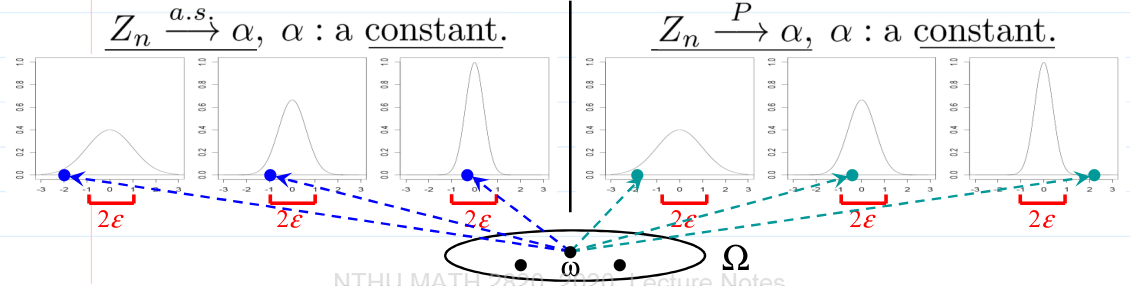
\includegraphics[width=0.9\textwidth]{image/converge1.png}
\end{figure*}

对于几乎必然收敛的情况,每个样本点上的序列随机变量都在逐渐趋近收敛变量;而对于依概率收敛的情况,由于对某个样本点的概率为0(例如连续随机变量),可能某一次样本点的序列随机变量接近收敛变量,下一次又远离收敛变量,只要保证总体概率趋近$1$即可。

\begin{theorem}[Borel-Cantelli定理]
    在概率空间 $(\Omega,\mathcal{F},\P)$中,设 $\{ A_n \in \mathcal{F} \}$,
    \begin{itemize}
        \item 若 $\sum_{n=1}^{\infty} \P(A_n) < \infty$, 则
        \[ \P(\limsup_{n \to \infty}A_n) = 0\]
        \item 若$\{ A_n \}$是独立事件列,且 $\sum_{n=1}^{\infty} \P(A_n) = \infty$, 则
        \[ \P(\limsup_{n \to \infty}A_n) = 1\]
    \end{itemize}
\end{theorem}

\begin{proposition}
    依概率收敛是几乎必然收敛的\underline{必要条件},但\underline{不是充分条件}。
\end{proposition}

\begin{example}[依概率收敛而不几乎必然收敛]
    设样本空间为$\Omega =(0,1]$,概率均匀分布在样本空间上,即$P([a,b])=b-a,0<a<b<1$。接下来对于$k \in \mathbb{N}_+$,将区间$(0,1]$分为$2^{k}$个等长的子区间,并分别记为$I_{k,j}=(\frac{j-1}{2^k},\frac{j}{2^k}]$。

    按以下方式定义随机变量序列$\{ X_n: \Omega \to \mathbb{R} \}$:
    \[ X_n(\omega)=\begin{cases}
            1, \omega \in I_{k,j}    \\
            0, \omega \notin I_{k,j} \\
        \end{cases} ,\quad n = 2^k+j-2\]
    同时定义随机变量$X: \Omega \to \mathbb{R}$为$X(\omega)=0,\forall \omega \in \Omega$

    由于
    \[ \P\{\omega \in \Omega: \abs{X_n(\omega) - X(\omega)}<\e\}=1-\frac1{2^k} \to 1 ,\quad \forall 0<\epsilon<1 \]
    所以$X_n \xrightarrow{\P} X$。
    然而对于任意$\omega \in \Omega$,无论$k$为何数,此次分割中,总有一个区间包含此样本点。即有无数个$X_i(\omega) = 1$。所以
    \[ \P\{ \omega \in \Omega: \lim_{n \to \infty}\abs{ X_n(\omega) - X(\omega)} < \epsilon \} =\P\{\emptyset \}=0 \]
    所以$X_n$不几乎必然收敛到$X$。
\end{example}

\begin{lemma}\label{lem:sum_product_CP}
    若$X_n \xrightarrow{\P} X, Y_n \xrightarrow{\P} Y$,则:
    \begin{enumerate}
        \item$X_n \pm Y_n \xrightarrow{\P} X \pm Y$
        \item$X_n Y_n \xrightarrow{\P} XY$
    \end{enumerate}
\end{lemma}
\begin{proof}
    \begin{enumerate}
        \item 因为
              \[ \{ \left\vert X_n+Y_n-X-Y \right\vert \ge \e \} \subset \{ \left\vert X_n-X \right\vert \ge \frac{\e}{2} \} \cup \{ \left\vert Y_n-Y \right\vert \ge \frac{\e}{2} \} \]
              所以
              \[ 0 \le P\{ \left\vert X_n+Y_n-X-Y \right\vert \ge \e \} \le P\{ \left\vert X_n-X \right\vert \ge \frac{\e}{2} \} + P\{ \left\vert Y_n-Y \right\vert \ge \frac{\e}{2} \} \]
              对上式取极限,并由夹逼定理得:
              \[ P\{ \left\vert X_n+Y_n-X-Y \right\vert \ge \e \}=0 \]
              由$Y_n \xrightarrow{\P} Y$易得$-Y_n \xrightarrow{\P} -Y$,所以又有$X_n - Y_n \xrightarrow{\P} X - Y$。
        \item 由于$2ab=(a+b)^2-a^2+b^2$,结合上一结论可知:$X_n Y_n \xrightarrow{\P} XY$的充分条件是$X_n \xrightarrow{\P} X \implies X_n^2 \xrightarrow{\P} X^2$。
              任取$\e >0$,有
              \begin{align*}
                  P\{|X_n^2-X^2| \ge \e \}= & P\{|X_n-X||X_n+X| \ge \e \}                         \\
                  =                         & P(\{|X_n-X||X_n+X| \ge \e \} \cap\{|X_n+X| \le M\}) \\
                                            & + P(\{|X_n-X||X_n+X| \ge \e \} \cap \{|X_n+X|>M\})  \\
                  \le                       & P\{|X_n-X| \ge \e / M\}+P\{|X_n+X|>M\}
              \end{align*}
              而
              \begin{align*}
                  P\{|X_n+X|>M\} \le & P\{|X_n-X|+|2X|>M\}                           \\
                  =                  & P(\{|X_n-X|+|2X|>M\} \cap\{|X_n-X|<1\})       \\
                                     & + P(\{|X_n-X|+|2X|>M\} \cap\{|X_n-X| \ge 1\}) \\
                  \le                & P\{|2 X|>M-1\}+P\{|X_n-X| \ge 1\}
              \end{align*}
              将$M$取足够大,使得对于任取的$\delta >0$,有$P\{ |X| >(M-1) / 2 \}< \delta$成立。并且由于$X_n \xrightarrow{\P} X$,所以
              \[ \exists N, \forall n>N \st P\{|X_n-X| \ge \e / M\},P\{|X_n-X| \ge 1\} < \delta \]
              综上
              \begin{align*}
                  P\{|X_n^2-X^2| \ge \e \} & \le P\{|X_n-X| \ge \e / M\}+P\{|X_n+X|>M\}                      \\
                                           & \le P\{|X_n-X| \ge \e / M\} + P\{|2 X|>M-1\}+P\{|X_n-X| \ge 1\} \\
                                           & < 3\delta
              \end{align*}
              即$X_n^2 \xrightarrow{\P} X^2$,所以$X_n Y_n \xrightarrow{\P} XY$
    \end{enumerate}
\end{proof}

\begin{theorem}
    若$X_n \xrightarrow{\P} X$,$g(x)$是$\mathbb{R}$上的连续函数,则$g(X_n) \xrightarrow{\P} g(X)$
\end{theorem}
\begin{proof}
    若$g_m(x)$是$m$次多项式函数,即$g_m(x)=\sum_{i=0}^m a_ix^i$,则由引理\ref{lem:sum_product_CP}知有
    \[ g_m(X_n) \xrightarrow{\P} g_m(X) \]
    因为$g(x)$是连续函数,所以可以用多项式函数去逼近$g(x)$,并且在任意有限区间上还是一致的,即对于任意$M,\e >0$,当$m$足够大的时候,存在$g_m(x)$,满足
    \[ \abs{g(x)-g_m(x)} < \e ,\ \abs x \le M \]

    接下来以$\abs X ,\abs{X_n} \le M$为界,将目标拆为两部分:
    \begin{align*}
            & P\{|g(X_n)-g(X)| \ge \e \}                                                                              \\
        =   & P(\{|g(X_n)-g(X)| \ge \e \}\cap \{\abs X ,\abs{X_n} \le M \})                                           \\
            & +P(\{|g(X_n)-g(X)| \ge \e \}\cap \{\{\abs X \le M\} \cup \{\abs{X_n} \le M\} \})                        \\
        \le & P(\{|g(X_n)-g(X)| \ge \e \}\cap \{\abs X ,\abs{X_n} \le M \}) + P\{\abs X \le M\}+ P\{\abs{X_n} \le M\}
    \end{align*}
    对于后半部分有:
    \[ \forall \delta >0 , \exists M >0 \st P\{\abs X \le M\},P\{\abs{X_n} \le M\}< \delta \]
    对于第一项,将$\{|g(X_n)-g(X)| \ge \e \}$拆分为三部分:
    \[ \{|g(X_n)-g(X)| \ge \e \} \subset \{|g(X_n)-g_m(X_n)| \ge \e / 3 \} \cup \{|g_m(X_n)-g_m(X)| \ge \e / 3 \} \cup \{|g_m(X)-g(X)| \ge \e / 3 \} \]
    又因为多项式函数逼近的一致性,稍加替换可得:
    \begin{align*}
        \left\{|g(X_n)-g_m(X_n)| \ge \e / 3 \right\}\cap\{|X| \le M\} \cap\left\{|X_n| \le M \right\} = & \emptyset \\
        \left\{|g_m(X)-g(X)| \ge \e / 3 \right\}\cap\{|X| \le M\} \cap\left\{|X_n| \le M \right\} =     & \emptyset
    \end{align*}
    所以
    \begin{align*}
            & P(\{|g(X_n)-g(X)| \ge \e \}\cap \{\abs X ,\abs{X_n} \le M \})                                     \\
        \le & P(\left\{|g_m(X_n)-g_m(X)| \ge \e / 3\right\} \cap\{|X| \le M\} \cap\left\{|X_n| \le M+1\right\}) \\
        \le & P\left\{|g_m(X_n)-g_m(X)| \ge \e / 3\right\}<\delta
    \end{align*}
    综上
    \[ P\{|g(X_n)-g(X)| \ge \e \} < 4 \delta\]
    即$g(X_n) \xrightarrow{\P} g(X)$
\end{proof}

\begin{note}
    相关证明技巧总结:对于事件$\{ |X+Y| > a+b \}$,有$\{ |X+Y| > a+b \} \subset \{ |X|>a \} \cup \{ |Y|>b \}$,从而有
    \[ P\{ |X+Y| > a+b \} \le P\{ |X|>a \} + P\{ |Y|>b \} \]
\end{note}

\subsection{依分布收敛}

\begin{definition}[依分布收敛]
    设随机变量$X, X_1, X_2, \dotsc$的分布函数分别为$F(x), F_1(x), F_2(x), \dotsc$。若对$F(x)$的任一\underline{连续点}$x$,都有
    \[ \lim_{n \to +\infty} F_n(x) = F(x) \]
    则称$\{ F_n(x) \}$\textbf{弱收敛}(converge weakly)于$F(x)$, 记作$F_n(x) \xrightarrow{W} F(x)$;也称$\{ X_n \}$\textbf{按分布收敛}(converge in distribution)于$X$,记作$X_n \xrightarrow{d} X$
\end{definition}
\begin{remark}
    对于非连续点,其收敛值可能使得收敛函数不满足分布函数特征(见下例),需要定义这些非连续点上的值,使其满足分布函数特征。
\end{remark}

\begin{example}
    设$\{ X_n \}$服从退化分布:
    \[ P \biggl(X_n = \frac1n \biggr) = 1, \quad n \in N_+\]
    其分布函数分别为:
    \[ F_n(x ) = \begin{cases}
            0, & x < 1/n,    \\
            1, & x \geq 1/n.
        \end{cases} \]
    因为$F_n(x)$是在点$x=1$处有跳跃,所以当$n \to +\infty$时,跳跃点位置趋于0。于是我们很自然地认为$\{ F_n(x) \}$应该收敛于点$x=0$处的退化分布,即
    \[ F(x) = \begin{cases}
            0, & x < 0,    \\
            1, & x \geq 0.
        \end{cases} \]
    但是,对任意的$n$,有$F_n(0) = 0$, 而$F(0) = 1$, 所以
    \[ \lim_{n \to +\infty} F_n(0) = 0 \neq 1 = F(0) \]
\end{example}

\begin{proposition}\label{prop:CP_VS_CD}
    依分布收敛是依概率收敛的\underline{必要条件},但\underline{不是充分条件}。但若依概率收敛到一个\underline{常数随机变量},则也可推出依分布收敛。
\end{proposition}
\begin{remark}
    直观来看,$X_n$依概率收敛到$X$,意味着$n$很大时,二者的距离大概率很近。那么随着$n$越来越大,$X_n$的行为自然会越来越像。对于某一区间$B$,样本点集$X^{-1}(B)=\{\omega\in\Omega : X(\omega) \in B\}$将与点集$X^{-1}_n(B)$越来越接近,其两随机变量出现在此区间的概率也将逐渐相等,这就是依分布收敛描述的东西。
\end{remark}
\begin{proof}
    \textbf{必要性}:设随机变量$X, X_1,  X_2, \dotsc$的分布函数分别为$F(x), F_1(x), F_2(x), \dotsc$。
    \begin{figure}[H]
        \centering
        \begin{subfigure}[]{0.8\textwidth}
            \centering
            
\includegraphics[width=\textwidth]{image/CP_to_CF1.jpg}
            \caption{$X_n>X$}
            \label{fig:CP_to_CF1}
        \end{subfigure}
        \begin{subfigure}[]{0.8\textwidth}
            \centering
            
\includegraphics[width=\textwidth]{image/CP_to_CF2.jpg}
            \caption{$X_n<X$}
            \label{fig:CP_to_CF2}
        \end{subfigure}
        %\caption{}
        \label{fig:CP_to_CF}
    \end{figure}
    如上图\ref{fig:CP_to_CF1},直观来看$P\{ X_n\le t \} \approx F(t-\e)$。而严格来看有:
    \begin{align*}
        F_n(t) & = P(X_n\le t)                                     \\
               & \ge P(X_n\le t,X\le t-\e)                         \\
               & =P(X\le t-\e) - P(X_n > t,X\le t-\e)              \\
               & \ge F(t-\e) - P(\left\vert X_n-X \right\vert >\e)
    \end{align*}
    数列$\{ F_n(t) \}$的极限未必存在,但可对两边取下极限得
    \[ F(t-\e) \leq \varliminf_{n \to +\infty} F_n(t) \]

    同理,如上图\ref{fig:CP_to_CF2},根据“对称性”,交换$X_n$与$X$的位置有:
    \[ F(t+\e) \ge F_n(t) - P(\left\vert X_n-X \right\vert >\e)\]
    对两边取下极限得
    \[ \varlimsup_{n \to +\infty} F_n(t) \leq  F(t+\e) \]

    综上有:
    \[ F(t-\e) \leq \varliminf_{n \to +\infty} F_n(t) \le \varlimsup_{n \to +\infty} F_n(t) \leq  F(t+\e) \]
    再令$\e \to 0+$得
    \[ F(t-0) \leq \varliminf_{n \to +\infty} F_n(t) \le \varlimsup_{n \to +\infty} F_n(t) \leq  F(t+0) \]
    所以当$t$为$F(x)$上的连续点时,$F(t-0)=F(t+0)$。根据夹逼定理,此时$\{ F_n(t) \}$的极限存在且
    \[ \lim_{n \to +\infty} F_n(x) = F(x) \]

    \textbf{充分性}(常数随机变量):设$X=c$,$c$为常数,其分布函数退化为:
    \[ F(x) = \begin{cases}
            0, & x < c,    \\
            1, & x \geq c.
        \end{cases} \]
    所以对任意的$\e > 0$, 有
    \begin{align*}
        P\{ \left\vert X_n-X \right\vert \ge \e \} & = P\{ X_n \geq c + \e \} + P\{ X_n \le  c - \e \}           \\
                                                   & \leq P\{ X_n > c + \frac{\e}{2} \} + P\{ X_n \le  c - \e \} \\
                                                   & = 1 - F_n(c + \e / 2 ) + F_n(c - \e ).
    \end{align*}
    由于$x = c + \e / 2$和$x = c - \e$均为$F(x)$的连续点,且$F_n(x) \stackrel{W}{\to} F(x)$,所以当$n \to +\infty$时,有
    \[ F_n(c + \e / 2 ) \to F(c + \e / 2 ) = 1, \quad F_n(c - \e) \to F(c - \e ) = 0 \]
    由此得
    \[ P\{ \left\vert X_n-X \right\vert \ge \e \} \to 0 \]
\end{proof}

\begin{example}[依分布收敛而不依概率收敛]
    设$X$的分布列为
    \[ P(X = -1 ) = \frac1{2}, \quad P(X = 1) = \frac1{2} \]
    令$X_n = -X$, 则$X_n$与$X$同分布。即$X_n$与$X$有相同的分布函数。故$X_n \stackrel{L}{\to} X$。

    但对任意$0 < \e < 2$,有
    \[ P\{ \left\vert X_n-X \right\vert \ge \e \} = P(2 \left\vert X \right\vert \geq \e ) = 1 \nrightarrow 0 \]
    即$X_n$不是依概率收敛于$X$。
\end{example}

\begin{figure}[H]
    \centering
    \begin{tikzpicture}
        \node[box](1) at(0,0) {几乎必然收敛};
        \node[box](2) at(4,0) {依概率收敛};
        \node[box](3) at(8,0) {按分布收敛};
        \draw[-to](1)--(2);
        \draw[-to](2)--(3);
        \draw[->,densely dotted](8,0.45) arc(0:180:2);
        \node at(6,1.5) {常数随机变量};
    \end{tikzpicture}
    \caption{三种收敛的关系}
    \label{fig:relationship_among_converges}
\end{figure}

\begin{theorem}[连续映射定理]\label{thm:continuous_mapping}
    设$g: \mathbb{R}^k \mapsto \mathbb{R}$为区间$B$上的\underline{连续}函数,并且$P(X \in B)=1$,则随机向量序列通过次映射后收敛情况与原先相同,即:
    \begin{align*}
        X_n^{(i)} \xrightarrow{\as} X^{(i)}  & \Rightarrow g(X_n^{(1)},\cdots X_n^{(k)}) \xrightarrow{\as} g(X^{(1)},\cdots X^{(k)}) \\
        X_n^{(i)} \xrightarrow{\P} X^{(i)}   & \Rightarrow g(X_n^{(1)},\cdots X_n^{(k)}) \xrightarrow{\P} g(X^{(1)},\cdots X^{(k)})  \\
        (X_n^{(i)}) \xrightarrow{d}(X^{(i)}) & \Rightarrow g(X_n^{(1)},\cdots X_n^{(k)}) \xrightarrow{d} g(X^{(1)},\cdots X^{(k)})   \\
    \end{align*}
\end{theorem}
\begin{proof}
    证明见书\cite[Asymptotic Statistics]{vaart_1998}中定理2.3。
\end{proof}

\begin{corollary}[Slutsky定理]\label{cor:Slutsky}
    若$X_n \xrightarrow{d} X, Y_n \xrightarrow{P} a$,其中$a$是常数,则:
    \begin{itemize}
        \item$Y_n X_n \xrightarrow{d} a X$
        \item$Y_n + X_n \xrightarrow{d} a + X$
        \item$\frac{X_n}{Y_n}  \xrightarrow{d} \frac{X}{a}$,若对所有的$n$都有$P(Y_n\neq 0)=1$,并且$a\neq 0$
    \end{itemize}
\end{corollary}
\begin{proof}
    由条件可知,$(X_n,Y_n) \xrightarrow{d}(X,a)$,且$g_1(X_n,Y_n)=X_n Y_n, g_2(X_n,Y_n)=X_n+Y_n, g_3(X_n,Y_n)=\frac{X_n}{Y_n}$都是连续函数($g_3$在定理中的限制下),所以仍然保持依分布收敛。
\end{proof}
\begin{remark}
    当$Y_n \xrightarrow{P} a$才能得出$(X_n,Y_n) \xrightarrow{d}(X,a)$;若$Y_n$依分布收敛到其他随机变量,则未必成立。
\end{remark}

\begin{theorem}[theta方法的极限定理]
    设
    \[ \frac{\sqrt{n}(X_n-\theta)}{\sigma} \xrightarrow{d} N(0,1) \]
    那么对于连续函数$g$,若$g'(\theta)\neq 0$存在,则
    \[ \frac{\sqrt{n}(g(X_n)-g(\theta))}{\sigma|g'(\theta)|} \xrightarrow{d} N(0,1) \]
\end{theorem}
\begin{proof}
    %TODO
\end{proof}

\begin{theorem}[连续性定理]\label{thm:continuity}
    设$F_n(x)$是一个累计函数序列,并且分别对应矩母函数$M_n(t)$;$F(x)$是一个累计函数,并且对应矩母函数$M(t)$。那么,$F(x)$的所有连续点上$F_n(x) \xrightarrow{M} F(x)$的充要条件是:
    \[ \forall t \in U(0,\delta) ,s.t. \lim_{n \to \infty}M_n(t) = M(t)\]
    其中$U(0,\delta)$代表某一包含零点的开区间。

    若矩母函数不存在,可替换成特征函数
    \[ \forall t \in \mathbb{R} ,\st \lim_{n \to \infty}\varphi_n(t) = \varphi(t)\]
\end{theorem}
\begin{remark}
    不能替换成密度函数或质量函数
\end{remark}

\begin{example}
    \textbf{离散情况}:
    设均匀随机变量$X_n \sim U(-\frac1{2},\frac1{2})$,那么$X_n \xrightarrow{d} 0$。然而$P_n(x) \to 0, \forall x \in \mathbb{R}$(不满足质量函数定义),并且$\lim_{n \to \infty}F_n(0)=\frac1{2}$(不满足累积函数定义)

    \textbf{连续情况}:
    设累积函数为$F_n(x)=x-\frac{\sin(2n\pi x)}{2n\pi}, 0<x<1$,那么$F_n \xrightarrow{d} U(0,1)$。然而$f_n(x)$无极限
\end{example}

\begin{example}[泊松分布收敛于正态分布]
    令$X_n \sim P(\lambda_n)$,并且$\lim_{n \to \infty}\lambda_n =\infty$。将变量标准化:
    \[ Z_n=\frac{X_n-\lambda_n}{\sqrt{\lambda_n}} \]
    那么
    \[M_{Z_n}(t)=\ee^{-t\sqrt{\lambda_n}}M_{X_n}(t)(\frac{t}{\sqrt{\lambda_n}})=\exp(-t\sqrt{\lambda_n}+\lambda_n(e^{\frac{t}{\sqrt{\lambda_n}}-1}))\]
    由于
    \[ \lim_{n \to \infty}\ln(M_{Z_n}(t))=\lim_{\lambda_n \to \infty}-t\sqrt{\lambda_n}+\lambda_n(e^{\frac{t}{\sqrt{\lambda_n}}-1})=\frac{t^2}{2} \]
    所以$Z_n \xrightarrow{d} N(0,1)$,即若$\lambda$很大,可通过$N(\lambda,\lambda)$估计$P(\lambda)$
\end{example}

\section{大数定理}\label{sec:large_number}

大数定律讨论的是在什么条件下,随机变量序列的算术平均依概率收敛到其均值
的算术平均。

\begin{definition}[大数定律的一般形式]\label{def:large_number_law}
    设有一随机变量序列$\{ X_n \}$,若满足:
    \[ \frac1n \sum_{i=1}^n X_i \xrightarrow{\P} \frac1n \sum_{i=1}^n E(X_i) \]
    则称该随机变量序列$\{ X_n \}$服从\textbf{大数定律}。
\end{definition}
\begin{note}
    柯西分布无均值、方差,不存在此定理。
\end{note}

不同的大数定律的差别只是对不同的随机变量序列$\{ X_n \}$而言, 有的是相互独立的随机变量序列, 有的是相依的随机变量序列, 有的是同分布的随机变量序列, 有的是不同分布的随机变量序列等等.

\begin{theorem}[切比雪夫大数定律]
    设$\{ X_n \}$为一列\underline{两两不相关}的随机变量序列,若每个$X_i$的\underline{方差存在,且有共同的上界},即$\Var(X_i) \le c ,\ i=1,2, \dotsc$,则$\{ X_n \}$服从大数定律\ref{def:large_number_law}。
\end{theorem}
\begin{remark}
    切比雪夫大数定律只要求$\{ X_n \}$互不相关, 并不要求它们是同分布的。假如$\{ X_n \}$是独立同分布的随机变量序列, 且方差有限, 则$\{ X_n \}$必定服从大数定律.
\end{remark}
\begin{proof}
    因为$\{ X_n \}$两两不相关,故
    \[ \Var \left(\frac1n \sum_{i=1}^n X_i \right) = \frac1{n^2} \sum_{i=1}^n\Var(X_i) \leq \frac{c}{n} \]
    再由切比雪夫不等式得:
    \[ P \left(\left\lvert \frac1n \sum_{i=1}^n X_i - \frac1n \sum_{i=1}^n E(X_i) \right\rvert \ge  \e \right) < \frac{\Var\left(\frac1n \sum_{i=1}^n X_i \right)}{\e^2} < \frac{c}{n\e^2} ,\quad \forall \e > 0 \]
    于是当$n \to +\infty$时,有
    \[ \lim_{n \to +\infty} P \left(\left\lvert \frac1n \sum_{i=1}^n X_i - \frac1n \sum_{i=1}^n E(X_i) \right\rvert < \e \right) = 1 \]
\end{proof}

\begin{theorem}[马尔可夫大数定律]
    对随机变量序列$\{ X_n \}$,若
    \[ \frac1{n^2}\Var \left(\sum_{i=1}^n X_i \right) \to 0 \]
    成立,则其服从大数定律。此条件被称为\textbf{马尔可夫条件}。
\end{theorem}
\begin{remark}
    马尔可夫条件对$\{ X_n \}$已经没有任何同分布、独立性、不相关的假定。证明过程与切比雪夫大数定律类似;切比雪夫大数定律显然可由马尔可夫大数定律推出。
\end{remark}

\begin{example}\label{ex:4.2.3}
    设$\{ X_n \}$为一同分布、方差存在的随机变量序列,且$X_n$仅与$X_{n-1}$和$X_{n+1}$相关,而与其他的$X_i$不相关。试问该随机变量序列$\{ X_n \}$是否服从大数定律?
\end{example}
\begin{solution}
    考虑其马尔可夫条件
    \[ \frac1{n^2}\Var \left(\sum_{i=1}^n X_i \right) = \frac1{n^2} \left[ \sum_{i=1}^n \Var(X_i) + 2 \sum_{i=1}^{n-1} \Cov(X_i, X_{i-1})\right] \]
    记$\Var(X_i) = \sigma^2$,则$\abs{\Cov(X_i, X_j)}\leq \sigma^2$,于是有
    \[ \frac1{n^2}\Var \left(\sum_{i=1}^n X_i \right) \leq \frac1{n^2} \left[n \sigma^2 + 2(n - 1) \sigma^2\right] \to 0 \]
    即马尔可夫条件成立, 故$\{ X_n \}$服从大数定律.
\end{solution}

\begin{theorem}[(辛钦)弱大数定理]
    设$\{ X_n \}$为一\underline{独立同分布}的随机变量序列,若$X_i$的数学\underline{期望存在}且为$\mu$,则$\{ X_n \}$服从大数定律,即:
    \[ \overline{X_n}=\frac1n\sum_{i=1}^n X_i \xrightarrow{\P} \mu \]
\end{theorem}
\begin{proof}
    因为$\{ X_n \}$同分布,故其特征函数相同,记为$\varphi(t)$。又因为$\varphi'(0)=i \E(X_i)$,则其位于$0$点附近的展开式为:
    \[ \varphi(t)=\varphi(0)+\varphi'(0)t+o(t)=1+i \mu t +o(t) \]
    由$\{ X_n \}$的独立性知$\overline{X_n}$的特征函数为:
    \[ \varphi_{\overline{X_n}}(t)=\left[ \varphi(\frac{t}{n}) \right]^n=\left[ 1+i \mu \frac{t}{n} +o(\frac{t}{n}) \right]^n \]
    对于任意$t$有:
    \[ \lim_{n \to \infty} \varphi_{\overline{X_n}}(t) = \ee^{i \mu t}\]
    再根据定理\ref{thm:continuity}与命题\ref{prop:CP_VS_CD},上述定理成立。
\end{proof}

\begin{example}[蒙特卡洛积分(平均值法)]
    为计算积分$I(f)=\int_0^1 f(x)\mathrm{d}x$,生成随机数$X_1,\cdots ,X_n \operatorname{i.i.d.} \sim U(0,1)$,并且计算$\hat{I}(f)=\overline{Y_n}, Y_i=f(X_n)$。由于$X_1,\cdots ,X_n \operatorname{i.i.d.}$,所以$Y_1,\cdots ,Y_n \operatorname{i.i.d.}$;并且$E(Y_i)=E(f(X_i))=\int_0^1 f(x)\cdot 1\mathrm{d}x=I(f)$,所以$\hat{I}(f)\xrightarrow{\P} E(Y_i)=I(f)$
\end{example}

\begin{example}[样本方差]\label{ex:sample_var}
    设随机变量$X_1,\cdots ,X_n \iid$,并且均值和方差分别为$\mu,\sigma$。令:
    \[ S_n^2=\frac1n\sum_{i=1}^n(X_i-\overline{X_n})^2 =(\frac1n\sum_{i=1}^nX_i^2)-\overline{X_n}^2 \]
    由于$g(x)=x^2$是连续函数,所以$\overline{X_n}^2 \xrightarrow{\P} \mu^2$。由于$X_1^2,\cdots X_n^2 \operatorname{i.i.d.}$,且$E(X_i^2)=\sigma^2+\mu^2$,所以$\overline{X_n^2} \xrightarrow{\P} \mu^2+\sigma^2$。因此:
    \[ S_n^2 \xrightarrow{\P}\mu^2+\sigma^2-\mu^2= \sigma^2 \]
\end{example}

\begin{example}\label{ex:t_disc_to_normal}
    若$X_n \sim t_n$,则$X_n \xrightarrow{d} N(0,1)$。
    令$Z \sim N(0,1),U_1,\cdots ,U_n \sim \chi^2_1$相互独立,则$\frac{Z}{\sqrt{(U_1+\cdots+U_n)/n}} \sim t_n$。由于$E(U_i)=1$,所以$\overline{U_n} \xrightarrow{\P} 1$,所以$\sqrt{\overline{U_n}} \xrightarrow{\P} 1$,所以$t_n=\frac{Z}{\sqrt{\overline{U_n}}} \xrightarrow{d} N(0,1)$(Slutsky定理\ref{cor:Slutsky})。
\end{example}

\begin{example}
    若$X_n \sim F_{m,n}$,则$mX_n \xrightarrow{d} \chi^2_m$。
    令$U \sim \chi^2_m,V_1,\cdots ,V_n \sim \chi^2_1$相互独立,则$\frac{U/m}{(V_1+\cdots+V_n)/n} \sim F_{m,n}$。由于$E(V_i)=1$,所以$\overline{V_n} \xrightarrow{\P} 1$,所以$mF_{m,n}=\frac{U}{\overline{V_n}} \xrightarrow{d} \chi^2_m$(Slutsky定理\ref{cor:Slutsky})。
\end{example}

大数定律讨论的是在什么条件下,随机变量序列的算术平均几乎必然收敛到其均值的算术平均。

\begin{definition}[强大数定律的一般形式]\label{def:strong_large_number_law}
    设有一随机变量序列$\{ X_n \}$,若满足:
    \[ \frac1n \sum_{i=1}^n X_i \xrightarrow{\as} \frac1n \sum_{i=1}^n E(X_i) \]
    则称该随机变量序列$\{ X_n \}$服从\textbf{强大数定律}。
\end{definition}

% \begin{theorem}[强大数定理]
%     设随机变量$X_1,\cdots ,X_n$相互独立,且$E(X_i)=\mu,\operatorname{Var}(X_i)=\sigma^2$,那么
%     \[ \overline{X_n}=\frac1n\sum_{i=1}^n X_i \xrightarrow{\as} \mu \]
% \end{theorem}



\section{中央极限定理}

中央极限定理讨论在什么条件下,独立随机变量和的分布函数会收敛到正态分布。

\subsection{独立同分布下的中心极限定理}

\begin{theorem}[林德伯格-莱维(Lindeberg-Levy)中央极限定理]\label{thm:central_limit_Classical}
    设随机变量$X_1,\cdots ,X_n,\operatorname{i.i.d.}$,且$E(X_i)=\mu,\operatorname{Var}(X_i)=\sigma^2$,令
    \[ \overline{X_n} = \frac1n\sum_{i=1}^n X_i, T_n=\sum_{i=1}^n X_i\]
    则:
    \[ \lim_{n \to \infty}P(\frac{T_n-n \mu}{\sigma\sqrt{n}}\le x)=\lim_{n \to \infty}P(\frac{\sqrt{n}(\overline{X_n}-\mu)}{\sigma}\le x) =\Phi(x)\]
    其中$\Phi(x)$是$N(0,1)$的累积函数,即:
    \[ \frac{T_n-n \mu}{\sigma\sqrt{n}}=\frac{\sqrt{n}(\overline{X_n}-\mu)}{\sigma} \xrightarrow{d} N(0,1)\]
\end{theorem}
\begin{proof}
    设$X_n - \mu$的特征函数为$\varphi(t)$。因为$E( X_n - \mu ) = 0 ,\ \Var(X_n - \mu ) = \sigma^2$, 所以有
    \[ \varphi'(0) = 0, \ \varphi''(0) = - \sigma^2 \]
    于是特征函数$\varphi(t)$有展开式
    \[ \varphi(t) = \varphi(0) + \varphi'(0) t + \varphi''(0) \frac{t^2}{2} + o(t^2)= 1 - \frac{1}{2} \sigma^2 t^2 + o(t^2) \]
    则$\{ Y_n^* \}$的特征函数为
    \[ \varphi_{Y_n^*}(t) = \left[ \varphi \biggl( \frac{t}{\sigma \sqrt{n}} \biggr) \right] ^n = \left[ 1 - \frac{t^2}{2n} + o \biggl( \frac{t^2}{n} \biggr) \right]^n  \]
    从而有
    \[ \lim_{n \to +\infty} \varphi_{Y_n^*}(t) = \ee^{-t^2/2} \]
    而$\ee^{-t^2/2}$正是$N(0,1)$分布的特征函数,根据定理\ref{thm:continuity},上述定理得证。
\end{proof}

\begin{example}[测量误差估计]
    假设每次测量结果为独立同分布的随机变量$X_1,\cdots ,X_n$, 其均值与方差分别为$\mu,\sigma^2$. 由中央极限定理可知$\frac{\sqrt{n}(\overline{X_n}-\mu)}{\sigma} \xrightarrow{d} N(0,1)$. 由例\ref{ex:sample_var}可知$S_n^2 \xrightarrow{\P} \sigma^2$, 即$\frac{\sigma}{S_n} \xrightarrow{\P} 1$(定理\ref{cor:Slutsky}). 所以:
    \[ \frac{\sqrt{n}(\overline{X_n}-\mu)}{S_n}=\frac{\sqrt{n}(\overline{X_n}-\mu)}{\sigma}\frac{\sigma}{S_n} \xrightarrow{d} N(0,1)\cdot 1=N(0,1) \]
    即可以通过分布$N(0,\frac{S_n^2}{n})$估计测量误差$\overline{X_n}-\mu$
\end{example}
\begin{remark}
    由定理\ref{thm:normal_sample_mean_variance}可知$\frac{\sqrt{n}(\overline{X_n}-\mu)}{S_n} \sim t_{n-1}$. 但由例\ref{ex:t_disc_to_normal}可知,$n\to \infty$时,$t$分布收敛于正态分布, 所以不冲突.
\end{remark}

\begin{corollary}[棣莫弗-拉普拉斯(de Moivre-Laplace)中心极限定理]
    若随机变量$X_1,\cdots ,X_n \operatorname{i.i.d.} \sim B(1,p)$, 则$T_n \sim B(n,p)$. 其中$E(T_n)=nE_(X_i)=np, \operatorname{Var}(T_n)=n\operatorname{Var}(X_i)=np(1-p)$。根据中央极限定理有:
    \[ \frac{T_n - np}{\sqrt{np(1-p)}} \xrightarrow{d} N(0,1) \]
    即当n很大时,$B(n,p)$可用$N(np,np(1-p))$近似。
\end{corollary}
\begin{remark}
    其他与二项分布一样, 可以通过独立同分布的随机变量相加得到的分布,也可在一定条件下近似为正态分布. 例如Gamma分布(可通过指数分布相加得到), 泊松分布(泊松分布相加), 负二项分布(几何分布相加), 参见图\ref{fig:relationship_among_univariate_distributions}
\end{remark}
\begin{remark}
    由定理\ref{thm:Poisson_theorem}可知,当$B(n,p)$中$n$很大$p$很小时,二项分布可近似为泊松分布;而泊松分布$\lambda$很大时,又可近似为正态分布。两者相比,一般在$p$较小时,用泊松分布近似较好;而在$np>5$和$n(1-p)>5$时,用正态分布近似较好。
\end{remark}

因为二项分布是离散分布,而正态分布是连续分布,所以用正态分布作为二项分布的近似计算中,作些修正可以提高精度。若$k_1 < k_2$均为整数,一般先作如下修正后再用正态近似$P(k_1 \leq T_n \leq k_2) = P(k_1 - 0.5 < T_n < k_2 + 0.5 )$。
\begin{example}
    若$T_n \sim b (25, 0.4)$,通过以下修正的正态近似得到$P(5 \leq \mu_n \leq 15)$:
    \begin{align*}
        P(5 \le T_n \le 15) & = P(5-0.5 < T_n < 15+0.5 )                                                                             \\
                            & \approx \Phi \biggl(\frac{15+0.5-10}{\sqrt{6}} \biggr) - \Phi \biggl(\frac{5-0.5-10}{\sqrt{6}} \biggr) \\
                            & = 2 \Phi (2.245) - 1 = 0.9754.
    \end{align*}
\end{example}

\subsection{独立不同分布下的中心极限定理}

设$\{ X_n \}$是一个相互独立的随机变量序列,它们具有有限的数学期望和方差:
\[ E(X_i) = \mu_i,\ \Var(X_i) = \sigma_i^2 \]
为讨论随机变量的和$Y_n = \sum_{i=1}^n X_i$,先将其标准化。由于
\begin{align*}
    E(Y_n)       & = \mu_1 + \mu_2 + \dotsb + \mu_n,                                         \\
    \sigma (T_n) & = \sqrt{\Var(X_i)} = \sqrt{\sigma_1^2 + \sigma_2^2 + \dotsb + \sigma_n^2}
\end{align*}
且记$\sigma(Y_n) = S_n$,则$Y_n$的标准化为
\[ Y_n^* = \frac{Y_n - (\mu_1 + \mu_2 + \dotsb + \mu_n)}{S_n} = \sum_{i=1}^n \frac{X_i - \mu_i}{S_n} \]

如果要求$Y_n^*$中各项$(X_i - \mu_i) / S_n$“均匀地小”,即对任意的$\tau > 0$,要求事件
\[ A_k = \left\{ \frac{\abs{X_i - \mu_i}}{S_n} > \tau \right\} = \bigl\{\abs{X_i - \mu_i} > \tau S_n \bigr\} \]
发生的可能性小,或直接要求其概率趋于0。为达到这个目的,要求
\[ \lim_{n \to +\infty} P \left\{ \max_{1 \leq i \leq n} \abs{X_i - \mu_i} > \tau S_n \right\} = 0. \]
因为
\[ P \left\{ \max_{1 \leq i \leq n} \abs{X_i - \mu_i} > \tau S_n \right\} = P \left\{ \cup_{i=1}^n (\abs{X_i - \mu_i} > \tau S_n) \right\} \leq \sum_{i=1}^n P(\abs{X_i - \mu_i} > \tau S_n) \]
不妨考虑
\[ P(\abs{X_i - \mu_i} > \tau S_n) = \E[\1(\abs{X_i - \mu_i} > \tau S_n)] \le \E[\frac{(x - \mu_i)^2}{\tau^2 S_n^2} \cdot \1(\abs{X_i - \mu_i} > \tau S_n)] \]
只要上式右侧之和趋于零,就可保证$Y_n^*$中各加项``均匀地小'',故有以下定义:

\begin{definition}[林德贝格条件]
    若$\{ X_n \}$是一个相互独立的随机变量序列,其均值与方差分别为$\mu_i,\sigma_i^2$。记$S_n=\sqrt{\sigma_1^2 + \sigma_2^2 + \dotsb + \sigma_n^2}$,若对任意的$\tau > 0$,有
    \[ \lim_{n \to +\infty} \frac{1}{\tau^2 S_n^2} \sum_{i=1}^n \E[(x - \mu_i)^2 \cdot \1(\abs{X_i - \mu_i} > \tau S_n)] = 0 \]
    则称$\{ X_n \}$满足\textbf{林德贝格条件}。
\end{definition}

\begin{theorem}[林德贝格中心极限定理]\label{thm:central_limit_Lindeberg}
    设独立随机变量序列$\{ X_n \}$满足林德贝格条件,则对任意的$x$,有
    \[ \lim_{n \to +\infty} P \left\{ \frac1{S_n} \sum_{i=1}^n (X_i - \mu_i) \leq x \right\} = \frac1{\sqrt{2\pi}} \int_{-\infty}^x \ee^{-t^2 /2 } \dd t \]
\end{theorem}

\begin{proposition}
    假如独立随机变量序列$\{ X_n \}$具有同分布和方差有限的条件,则必定满足林德贝格条件。也就是说定理\ref{thm:central_limit_Classical} 是定理~\ref{thm:central_limit_Lindeberg} 的特例。
\end{proposition}
\begin{proof}
    设连续随机变量序列$\{ X_n \}$独立同分布,其密度函数、均值、方差分别为为$f(x),\mu_i = \mu ,\sigma_i = \sigma$。这时$S_n = \sigma \sqrt{n}$,由此得
    \[ \frac{1}{S_n^2} \sum_{i=1}^n \int_{\abs{x_i - \mu_i} > \tau S_n} (x - \mu_i)^2 f(x) \dd x = \frac{n}{n \sigma^2} \int_{\abs{x - \mu} > \tau \sigma \sqrt{n}} (x - \mu)^2 f(x) \dd x. \]
    因为方差存在,即
    \[ \Var(X_i) = \int_{-\infty}^{+\infty} (x - \mu)^2 f(x) \dd x < + \infty. \]
    所以其尾部积分一定有
    \[ \lim_{n \to +\infty} \int_{\abs{x - \mu} > \tau \sigma \sqrt{n}} (x - \mu)^2 f(x) \dd x = 0, \]
    故林德贝格条件满足。
\end{proof}

林德贝格条件虽然比较一般,但该条件较难验证,下面的李雅普诺夫条件则比较容易验证,因为它只对矩提出要求,因而便于应用。

\begin{theorem}[李雅普诺夫中心极限定理]
    设$\{ X_n \}$为独立随机变量序列,若存在$\delta > 0$,满足
    \begin{equation}\label{eq:4.4.5}
        \lim_{n \to +\infty} \frac{1}{S_n^{2 + \delta}} \sum_{i=1}^n \E \bigl(\abs{X_i - \mu_i}^{2+\delta} \bigr) = 0,
    \end{equation}
    则对任意的$x$, 有
    \[ \lim_{n \to +\infty} P \biggl\{ \frac{1}{S_n} \sum_{i=1}^n \bigl( X_i - \mu_i \bigr) \leq x \biggr\} = \frac{1}{\sqrt{2\pi}} \int_{-\infty}^x \ee^{-t^2/2} \dd t \]
    其中$\mu_i$与$S_n$如前所述.
\end{theorem}

\begin{table}[h]
    \centering
    \begin{tabular}{@{}cccc@{}}
        \toprule
                   & 大数定律                                                           & 强大数定律   & 中心极限定理     \\ \midrule
        收敛       & 依概率收敛                                                         & 依概率1收敛  & 依分布收敛       \\
        伯努利实验 & 伯努利                                                             & 博雷尔       & 棣莫弗-拉普拉斯 \\
        独立同分布 & 辛钦                                                               & 科尔莫戈罗夫 & 林德伯格-莱维   \\
        一般场合   & \begin{tabular}[c]{@{}c@{}}泊松\\ 切比雪夫\\ 马尔可夫\end{tabular} & 科尔莫戈罗夫 & 林德伯格-费勒   \\ \bottomrule
    \end{tabular}
\end{table}

\begin{problemset}[错题记录]
    \item (茆4.1.2)
    \item (茆4.3.4)在伯努利试验中, 事件$A$出现的概率为$p$, 令
    \[ X+n = \begin{cases}
            1, & \text{若在第} \ n \ \text{次及第} \ n+1 \ \text{次试验中} \ A \ \text{出现} \\
            0, & \text{其他}.
        \end{cases} \]
    证明$\{ X_n \}$服从大数定律.
    \item (茆4.3.12)(伯恩斯组大数定律) 设$\{ X_n \}$是方差有界的随机变量序列, 且当$\lvert k - l \rvert \to +\infty$时, 一致地有$\Cov(X_k, X_l) \to 0$, 证明$\{ X_n \}$服从大数定律.
    \item (茆4.3.13)(格涅坚科大数定律) 设$\{ X_n \}$是随机变量序列, 若记
    \[ Y_n = \frac{1}{n} \sum_{i=1}^n X_i, \ a_n = \frac{1}{n} \sum_{i=1}^n E (x_i) \]
    则$\{ X_n \}$服从大数定律的充要条件是
    \[ \lim_{n \to +\infty} E \left( \frac{( Y_n - a_n )^2}{1 + ( Y_n - a_n )^2} \right) = 0 \]
    \item (茆4.3.14)设$\{ X_n \}$为独立同分布的随机变量序列, 方差存在。又设$\sum_{n=1}^{+\infty} a_n$为绝对收敛级数。令$Y = \sum_{i=1}^n X_i$, 证明$\{ a_n Y_n \}$服从大数定律。
    \item (茆4.3.16)设$\{ X_n \}$为独立同分布的随机变量序列, 其方差有限, 且$X_n$不恒为常数。如果$S_n = \sum_{i=1}^n X_i$, 试证: 随机变量序列$\{ S_n \}$不服从大数定律.
    \item (李5.25)
    \item (李5.45)
    \item (李5.46)
    \item (李5.60)
\end{problemset}